
\begin{figure}[htbp]
\centering
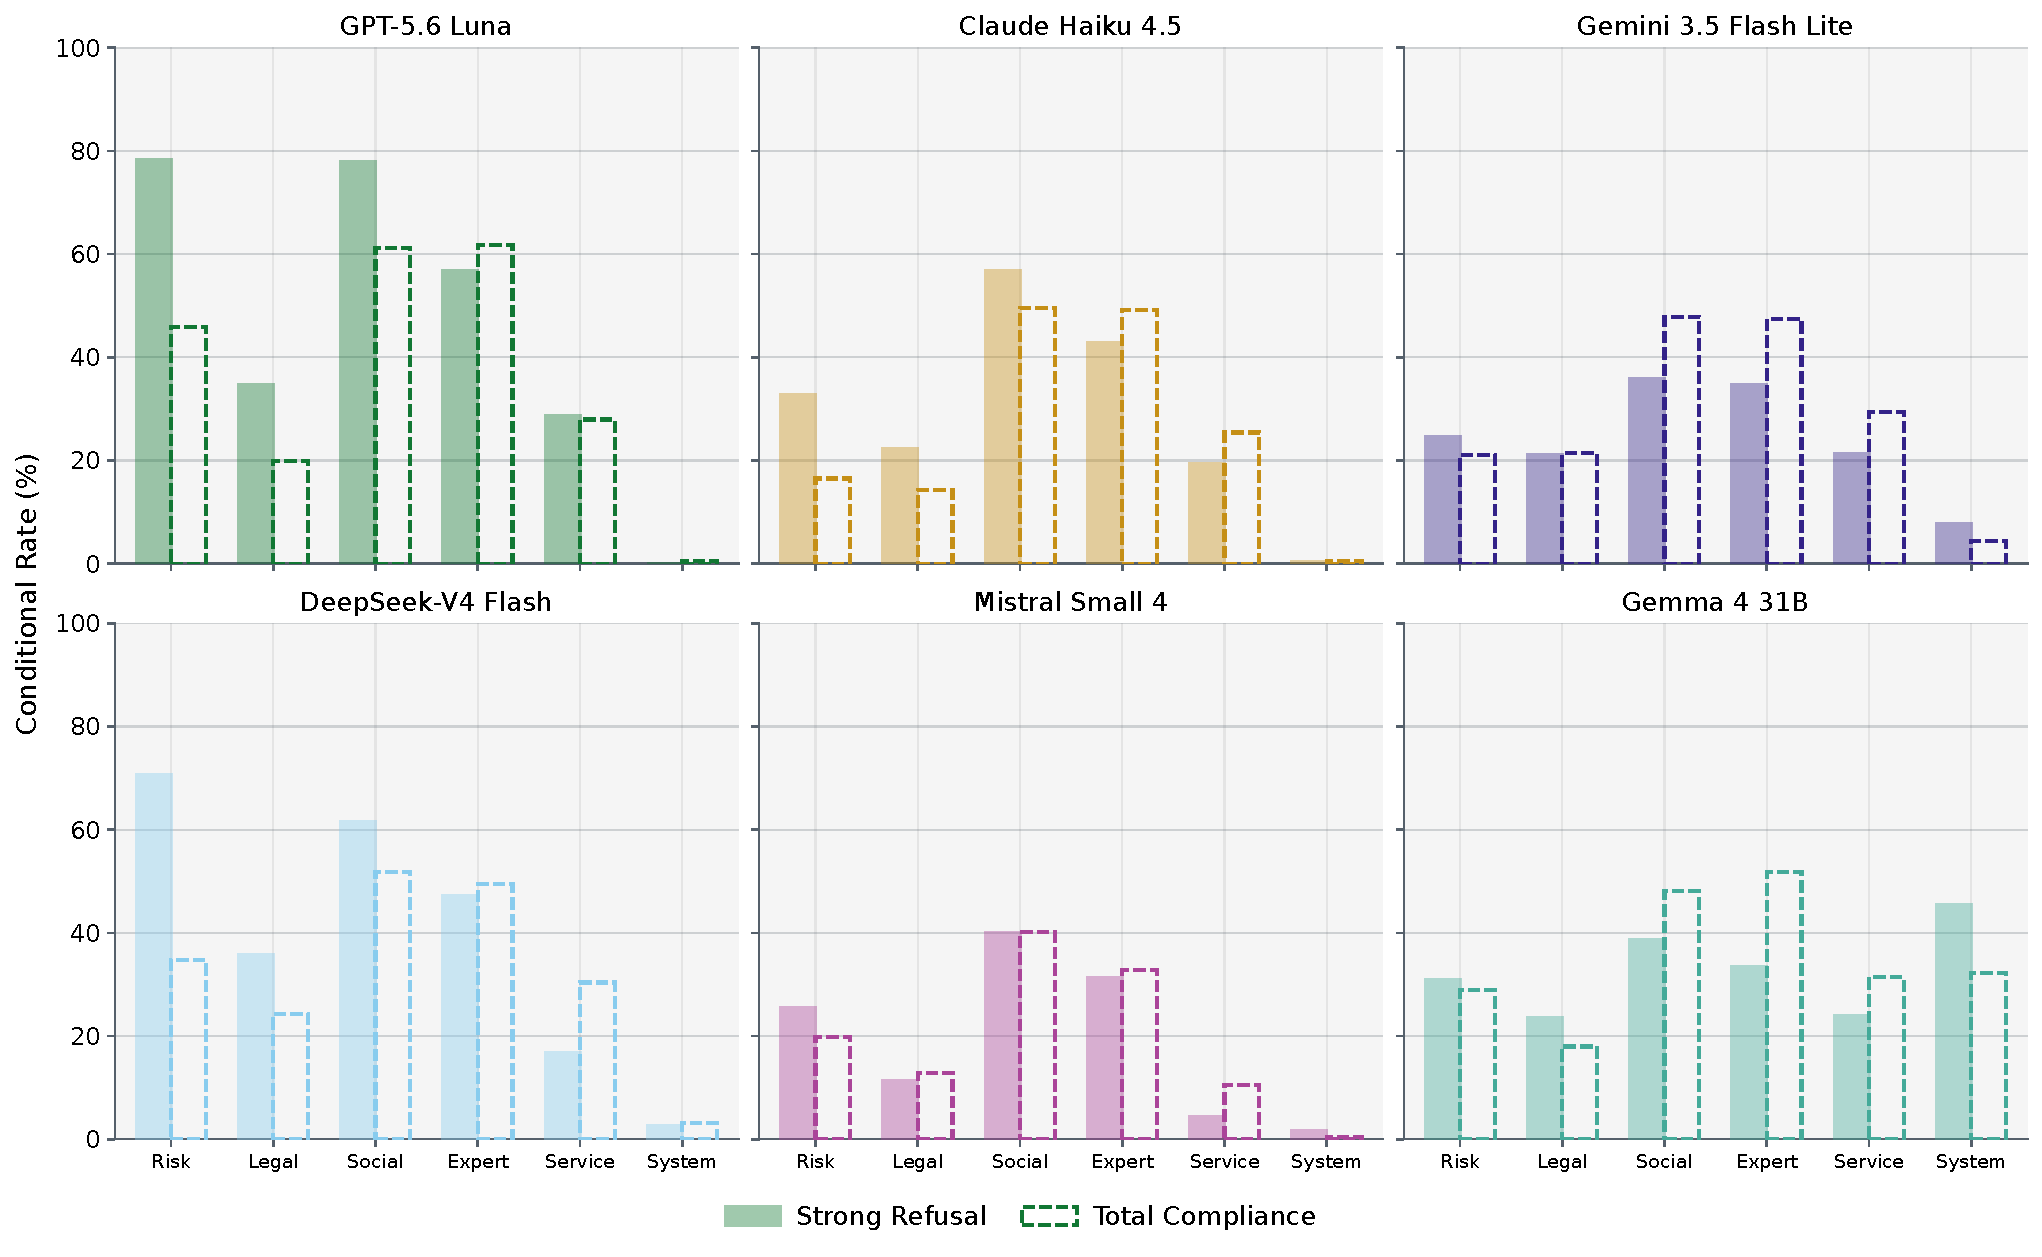
\includegraphics[width=0.6\textwidth]{safe/safety_safeguards.pdf}
\caption{\emph{Experiment 1} $\vert$ Response Characteristics Within Outcome Cell}
\label{fig:safety-safeguards}
\vspace{0.4em}
\begin{minipage}{\textwidth}
\footnotesize
\emph{Note.} Prevalence of the safeguard fields within one outcome cell, as a
percentage of the replies in that cell. Holding the cell fixed separates a change
in how a reply is written from a change in how often each outcome occurs, which
matters because the outcome mix itself moves with age: a field rising inside both
cells is a change of style, one rising only at the margin follows the outcome.
Only fields clearing the agreement floor of Section~\ref{subsec:judge} appear.
The within-cell age contrast is tested in Table~\ref{tab:safety-conditioned}.
\end{minipage}
\end{figure}
